\chapter{Fundamentos}

\section{Medidas de precisión en traducción}

\section{Transformers}
La aparición de la arquitectura \textbf{transformer}, introducida por \textit{Vaswani et al.} \cite{vaswani2023attentionneed}, supuso un cambio de paradigma en el procesamiento de secuencias, desplazando a las redes recurrentes en tareas de modelado de lenguaje. La relevancia de este modelo en el presente trabajo radica en su capacidad para gestionar dependencias de largo alcance mediante el mecanismo de auto-atención (\textit{self-attention}), el cual permite que cada elemento de una secuencia (ya sea una palabra o un \textit{keypoint} del cuerpo) sea procesado en relación con todos los demás de forma paralela. Por ello, dedicaremos esta sección a entender el funcionamiento de los \textit{transformers} con cierto nivel de detalle.

\subsection{¿Por qué Transformers?}
Para entender la relevancia e inovación de los transformers es necesario conocer lo que les precedía. En particular, las \textit{long short-term memory} y las \textit{gated recurrent neural networks} dominaron el procesamiento de secuencias mediante mecanismos de computación recurrente, los cuales procesan la información de manera secuencial siguiendo el orden temporal de la entrada. Estas arquitecturas presentaban dos limitaciones fundamentales: la dificultad para captar dependencias de largo alcance debido al desvanecimiento del gradiente y la imposibilidad de paralelizar el entrenamiento, lo que restringe enormemente la eficiencia computacional con secuencias largas.

Los transformers proponen abandonar por completo la recurrencia en favor del mecanismo de atención, lo que les permite captar dependencias de largo alcance en los textos de forma directa y con operaciones fácilmente paralelizables. En lugar de procesar la secuencia elemento a elemento, estos modelos consideran simultáneamente todos los tokens de entrada mediante el mecanismo de auto-atención, que calcula la relevancia relativa entre cada par de posiciones de la secuencia.

Este enfoque introduce varias ventajas clave. En primer lugar, elimina la dependencia estrictamente secuencial del cómputo, permitiendo un uso mucho más eficiente del hardware moderno, especialmente en arquitecturas paralelas como las \textbf{GPUs}. En segundo lugar, facilita el modelado de relaciones a larga distancia sin los problemas asociados al desvanecimiento del gradiente, ya que cualquier elemento de la secuencia puede interactuar directamente con cualquier otro en un solo paso de atención.

Además, los transformers incorporan mecanismos como las codificaciones posicionales para preservar la información sobre el orden de la secuencia, compensando así la ausencia de recurrencia. Esta combinación de atención global y representación posicional ha demostrado ser altamente efectiva en tareas de modelado del lenguaje y traducción automática, superando ampliamente a las arquitecturas recurrentes tradicionales.

Es natural plantearse si esta habilidad y facilidad que presentan los transoformers en la traducción de lenguajes se translada a la lengua de signos utilizando los \textit{keypoints} como representación de los signos.

\subsection{Codificación Posicional} % \textit{Positional Encoding}}

\subsection{Mecanismo de Auto-atención} % \textit{Self-Attention Mechanism}
La función de atención es un mecanismo que permite a un modelo identificar y priorizar la información más relevante dentro de un conjunto de datos. Para ello, compara una consulta, \textit{query} con un conjunto de claves, \textit{keys}, mediante una función de compatibilidad, que mide qué tan bien coincide la \textit{query} con cada \textit{key}, generando pesos que reflejan la importancia de cada elemento. Con base en estos pesos, se calcula una combinación ponderada de los valores \textit{values}, produciendo así una representación que enfatiza los componentes más pertinentes.

La función de atención más relevante es la \textit{Scaled Dot-Product Attention} cuya entrada son claves y consultas de dimensión $d_k$ y valores de dimensión $d_v$. En la práctica sacando provecho de que la multiplicación entre matrices está muy optimizada estas operaciones se hacen mediante matrices, obteniendo la siguiente fórmula.
\begin{equation*}
Attention(Q,K,V) = softmax\left( \frac{QK'}{\sqrt{d_k}}\right)V.
\end{equation*} Se añade el factor de escalado $\sqrt{d_k}$ pues si las matrices de \textit{query} y \textit{key} son de una muy alta dimensión, es posible que los valores exploten en tamaño donde la función \textit{softmax} se vuelve muy ``extrema'', es decir, asigna casi todo el peso a un solo elemento y hace que los gradientes sean muy pequeños, dificultando el entrenamiento.
\begin{figure}[H]
\center
\begin{tikzpicture}[
    % Estilo base
    block/.style={
        rectangle,
        draw=black,
        line width=1.5pt,
        rounded corners=2pt,
        minimum width=2.5cm,
        minimum height=0.8cm,
        font=\sffamily\Large,
        align=center
    },
    % Cambiamos 'scale' por 'styleScale' para evitar el error de pgfkeys
    styleMatmul/.style={block, fill=blue!15!purple!20},
    styleScale/.style={block, fill=yellow!25},
    styleMask/.style={block, fill=red!15},
    styleSoftmax/.style={block, fill=green!15},
    arrow/.style={-Stealth, line width=1.2pt}
]

    % --- NODOS ---
    \node (Q) at (0,0) {\sffamily\Large Q};
    \node (K) at (2,0) {\sffamily\Large K};
    \node (V) at (4,0) {\sffamily\Large V};

    % Columna central (usando el nuevo nombre de estilo styleScale)
    \node[styleMatmul, above=0.8cm of $(Q)!0.5!(K)$] (mm1) {MatMul};
    \node[styleScale, above=0.6cm of mm1] (sc) {\text{Scale}};
    \node[styleMask, above=0.6cm of sc] (mask) {Mask (opt.)};
    \node[styleSoftmax, above=0.6cm of mask] (sm) {SoftMax};

    % Bloque superior
    \node[styleMatmul, minimum width=4cm, above=0.8cm of sm, xshift=1.4cm] (mm2) {MatMul};

    % Salida
    \node (out) [above=0.7cm of mm2] {};

    % --- CONEXIONES ---
    \draw[arrow] (Q.north) -- ([xshift=-1cm]mm1.south);
    \draw[arrow] (K.north) -- ([xshift=1cm]mm1.south);
    \draw[arrow] (mm1) -- (sc);
    \draw[arrow] (sc) -- (mask);
    \draw[arrow] (mask) -- (sm);
    \draw[arrow] (sm.north) -- ([xshift=-1.4cm]mm2.south);
    \draw[arrow] (V.north) -- ([xshift=1.6cm]mm2.south);
    \draw[arrow] (mm2.north) -- (out);

\end{tikzpicture}
\caption{Una cabeza de atención}
\end{figure}







\shorthandoff{<}
\shorthandoff{>}
\begin{figure}[H]
\center
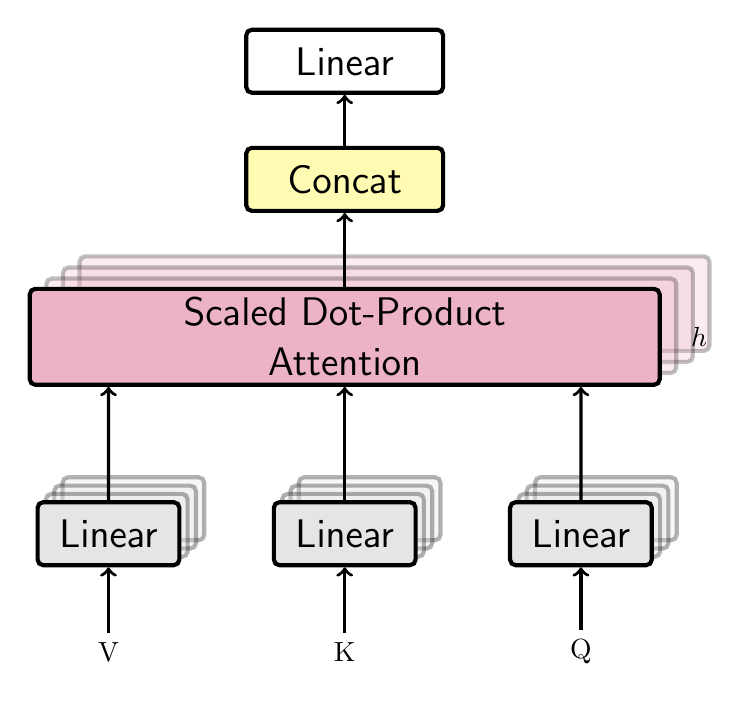
\begin{tikzpicture}[
    box/.style={
        rectangle,
        draw=black,
        line width=1.5pt,
        rounded corners=2pt,
        minimum width=2.5cm,
        minimum height=0.8cm,
        font=\sffamily\Large,
        align=center
    },
    smallbox/.style={
        rectangle,
        draw=black,
        line width=1.5pt,
        rounded corners=2pt,
        minimum width=1.8cm,
        minimum height=0.8cm,
        font=\sffamily\Large,
        align=center
    },
    arrow/.style={->, line width=1.2pt},
]

% Inputs
\node (V) at (-3,0) {V};
\node (K) at (0,0) {K};
\node (Q) at (3,0) {Q};


% === STACKED BACKGROUND (dibujar primero) ===
\foreach \i in {3,2,1} {
    \node[box, fill=purple!30,
        minimum width=8cm, minimum height=1.2cm, xshift=\i*6pt, yshift=\i*4pt, opacity=0.25] (att_box_\i) at (0,4) {};
    \node[smallbox, fill=gray!20,
          xshift=\i*3pt, yshift=\i*3pt, opacity=0.3] at (-3,1.5) {};
    \node[smallbox, fill=gray!20,
          xshift=\i*3pt, yshift=\i*3pt, opacity=0.3] at (0,1.5) {};
    \node[smallbox, fill=gray!20,
          xshift=\i*3pt, yshift=\i*3pt, opacity=0.3] at (3,1.5) {};
}

% === MAIN (dibujar al final, encima) ===
\node[box, fill=purple!30, minimum width=8cm] (attn) at (0,4)
{Scaled Dot-Product\\Attention};

% Linear layers
\node[smallbox, fill=gray!20] (linV) at (-3,1.5) {Linear};
\node[smallbox, fill=gray!20] (linK) at (0,1.5) {Linear};
\node[smallbox, fill=gray!20] (linQ) at (3,1.5) {Linear};

\node[box, fill=yellow!30] (concat) at (0,6) {Concat};
\node[box] (linear) at (0,7.5) {Linear};

% Arrows
\draw[arrow] (V) -- (linV);
\draw[arrow] (K) -- (linK);
\draw[arrow] (Q) -- (linQ);

\draw[arrow] (linV.north) -- ([xshift=-3cm]attn.south);
\draw[arrow] (linK.north) -- (attn.south);
\draw[arrow] (linQ.north) -- ([xshift=3cm]attn.south);

\draw[arrow] (attn) -- (concat);
\draw[arrow] (concat) -- (linear);

% h label
\node at (4.5,4) {$h$};

\end{tikzpicture}
\end{figure}
\shorthandon{<}
\shorthandon{>}

